\section{Wikiaves x SpeciesLink}

\texto

\subsection{Registros}

\begin{figure}[h!]
\centering
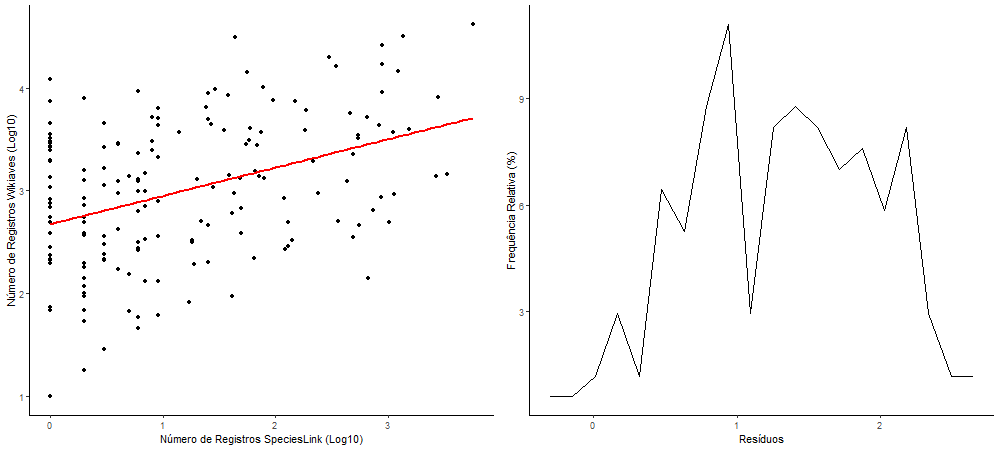
\includegraphics[width = 12cm]{Imagens/4113.png}
\\{\scriptsize  Figura 19: Relação linear entre o número de registros (Log10) nos bancos de dados SLI e WAV2 pareados por X municípios redundantes e respectiva distribuição de resíduos (direita, em unidades de desvio-padrão). Outliers bivariados foram excluídos. n = 171, r2 = 0,1588, P < 0,0001 .}
\end{figure}

\texto

\subsection{Espécies}

\begin{figure}[h!]
\centering
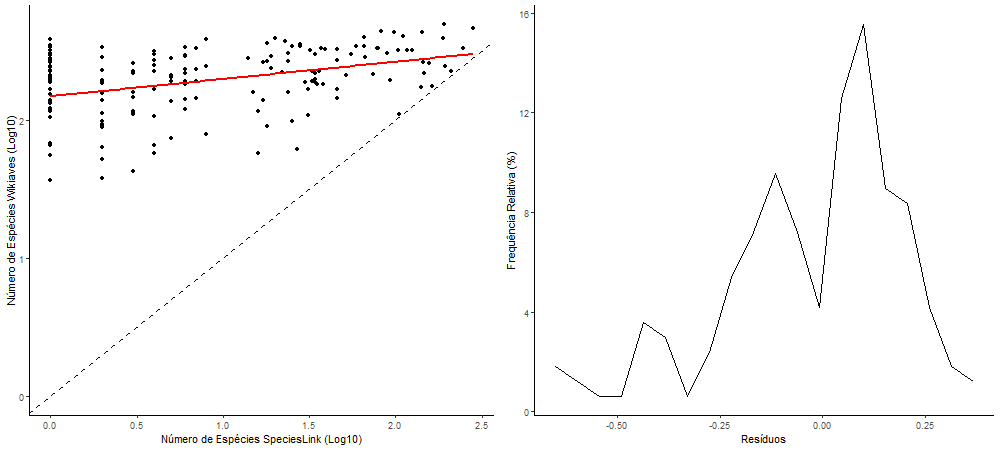
\includegraphics[width = 12cm]{Imagens/4213.png}
\\{\scriptsize Figura 20: Relação linear entre o número de espécies (Log10) nos bancos de dados SLI e WAV2 pareados por X municípios redundantes e respectiva distribuição de resíduos (direita, em unidades de desvio-padrão). Outliers bivariados foram excluídos. n = 167 , r2 = 0,1523 , P < 0,0001 .}
\end{figure}

\subsection {Registros x Espécies}

\begin{figure}[h!]
\centering
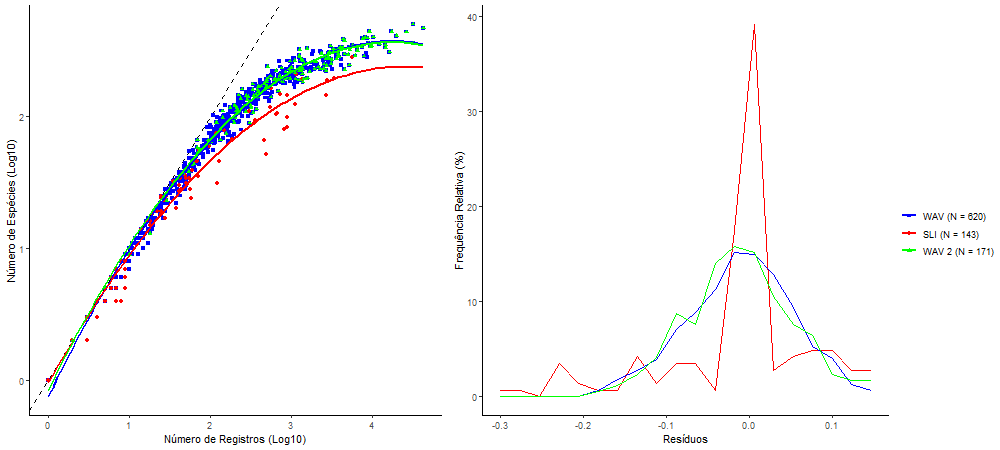
\includegraphics[width = 15cm]{Imagens/4333.png}
\\{\scriptsize Figura 21: Relação quadrática entre o número de espécies e o número de registros (ambos em Log10) nos bancos de dados WAV, SLI e WAV2 pareados por município e respectiva distribuição de resíduos (direita, em unidades de desvio-padrão). Outliers bivariados foram excluídos. n = 620, r2 = 0,9875, P < 0,0001 no Wikiaves. n = 143, r2 = 0,9867, P < 0,0001 no Wikiaves. n = 171, r2 = 0,9647, P < 0,0001 no Wikiaves 2.}
\label{Figura 20}
\end{figure}

\newpage
